
\chapter{Methodology}

\section{Process Model}
The team is following the Agile process model for the development of TRIBAL. Agile
was chosen because it allows the project to be broken down into small, manageable parts
called sprints, and each sprint produces a working piece of the application. This is useful
for a minor project because requirements can be refined as the team learns more, and
progress can be shown at regular intervals like this mid-term defense.
The project has been divided into the following sprints:
\begin{itemize}
\item Sprint 1: Project setup, requirement analysis, and UI/UX wireframing in Figma.
\item Sprint 2: Flutter onboarding flow, authentication screens (Login and Signup), and
post-signup profile completion screens.
\item Sprint 3: Django backend setup, PostgreSQL database design, and JWT-based
authentication APIs.
\item Sprint 4: Design and implementation of the roommate compatibility scoring
algorithm (current sprint).
\item Sprint 5: Real-time chat system using Django Channels and WebSockets.
\item Sprint 6: Event creation and joining module.
\item Sprint 7: Integration testing between the Flutter frontend and Django backend.
\item Sprint 8: Final testing, bug fixing, and documentation.
\end{itemize}
At the time of this report, the team has completed Sprints 1 to 4 and has started work on
Sprint 5.

\begin{figure}[H]
    \centering
    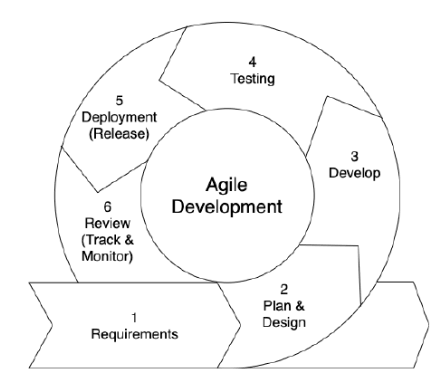
\includegraphics[width=0.8\textwidth]{images/process.png}
    \caption{Agile Process Model}
    \label{fig:agile_process}
\end{figure}


\section{System Block Diagram}

\begin{figure}[H]
    \centering
    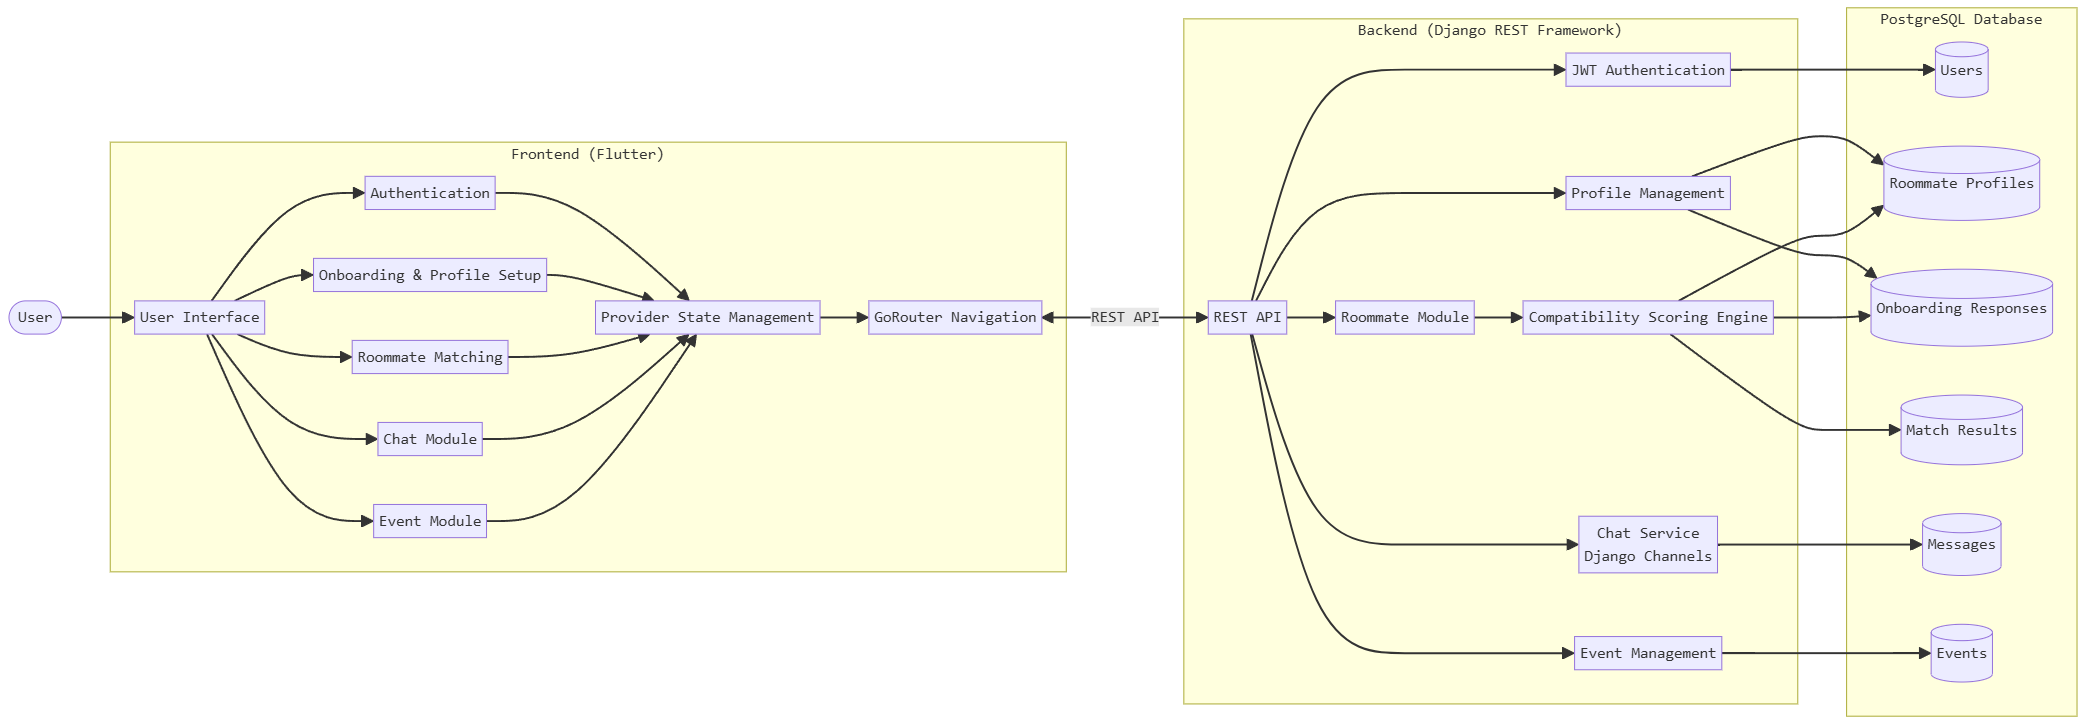
\includegraphics[width=0.8\textwidth]{images/system.png}
    \caption{System Block Diagram}
    \label{fig:block_diagram}
\end{figure}
The system is divided into three main layers:
\begin{itemize}
\item Frontend (Flutter): Handles the user interface, including onboarding,
authentication screens, and profile setup. The frontend uses Provider for state
management, GoRouter for navigation, and follows an MVC-based architecture.
\item Backend (Django): Exposes REST APIs for authentication, user profiles, and
roommate matching. The roommate matching logic lives entirely inside a single
roommate module, which keeps the matching-related code organized and separate
from the rest of the backend.
\item Database (PostgreSQL): Stores user accounts, roommate profile data, and
onboarding responses that are later used by the scoring algorithm.
\end{itemize}
The Flutter app communicates with the Django backend through REST APIs. JWT
tokens are used to keep the user logged in and to secure each API request. When a user
requests roommate matches, the request goes to the roommate module, which fetches
relevant profiles from the database, runs the scoring algorithm, and returns a ranked list
of compatible roommates back to the app.


\section{Algorithm}

\subsection{Roommate Compatibility Scoring Algorithm}
The core feature of TRIBAL at this stage is the roommate compatibility scoring
algorithm. The team decided not to use machine learning for this feature. Instead, a rule-based weighted scoring system was designed. This decision was made because a rule-based system is easier to explain, easier to test, and does not need a large dataset to train
on, which makes it more suitable for a minor project than a machine learning model.
The algorithm compares two users’ onboarding answers and produces a single
compatibility score between 0 and 100. The onboarding answers used in scoring include
cleanliness, budget, sleep schedule, noise level, smoking, guests, interests, study habit,
food preference, and drinking habit. The pet preference field is collected during
onboarding and stored in the profile, but it is not currently used in the scoring calculation.
Each factor is given a weight depending on how much it usually affects roommate
compatibility in real life. For ex le, cleanliness and budget are given higher weights
because mismatches in these areas are more likely to cause conflict, while smaller
lifestyle preferences are given lower weights.

Table 3.1 below shows the weight distribution used in the scoring algorithm.
\begin{table}[H]
\centering
\begin{tabular}{|l|c|}
\hline
\textbf{Factor} &  \textbf{Weight (\%)} \\
\hline
Cleanliness & 15 \\
Budget & 15 \\
Sleep Schedule & 12 \\
Noise Level & 10 \\
Smoking & 10 \\
Guests & 8 \\
Interests & 10 \\
Study Habit & 8 \\
Food Preference & 7 \\
Drinking & 5 \\
\hline
\end{tabular}
\caption{Compatibility Scoring Weights}
\label{table:scoring_weights}
\end{table}
The general formula used to calculate the final compatibility score is:

\begin{equation}
\text{Final Score} = \sum \left(\text{Factor Match Value} \times \text{Factor Weight}\right)
\end{equation}

Where Factor Match Value is a number between 0 and 1 that represents how closely two
users’ answers match for a particular factor, and Factor Weight is the percentage weight
assigned to that factor as shown in Table 3.1.
For factors with a small number of fixed options, such as smoking or sleep schedule, the
match value is calculated using a simple rule: if both users selected the same option, the
match value is 1; if their answers are close but not the same (for ex le, “early riser”
and “no preference”), a partial match value such as 0.5 is given; and if the answers
directly conflict (for ex le, “smoker” matched with “non-smoker, no smoking
allowed”), the match value is set to 0.
For factors that involve multiple selections, such as interests, the match value is
calculated as the number of common interests divided by the total number of unique
interests selected by both users combined. This gives a percentage overlap between the
two users’ interests.
For numeric factors like budget, the match value decreases as the difference between the
two users’ stated budgets increases. If the difference is within an acceptable range, the
match value stays close to 1. If the difference is very large, the match value moves closer
to 0.


\subsection{Deal Breakers}
Apart from the weighted scoring, the algorithm also includes a deal breaker check. Some lifestyle differences are considered serious enough that they should not simply lower the score a little, but should instead strongly affect or override the final match. For ex le, if one user is a heavy smoker and the other has explicitly said they cannot live with a smoker at all, this is treated as a deal breaker rather than just a normal mismatch. Table 3.2 lists the deal breaker rules currently used in the algorithm.
\begin{table}[H]
\centering
\begin{tabular}{|l|l|}
\hline
\textbf{Condition}  & \textbf{Effect on Score} \\
\hline
Smoking conflict (smoker vs. strictly non-smoking) & Score capped at a low maximum \\
Extreme budget mismatch (outside acceptable range) & Score capped at a low maximum \\
Opposite cleanliness extremes (very messy vs. very strict) & Score significantly reduced \\
\hline
\end{tabular}
\caption{Deal Breaker Rules}
\label{table:deal_breakers}
\end{table}
When a deal breaker condition is detected, the algorithm does not let the final score go above a fixed low ceiling, even if all other factors match well. This makes sure that users are not shown as highly compatible with someone they have a fundamental lifestyle conflict with.


\subsection{Final Score Calculation}
Once all the individual factor match values are calculated and weighted, they are added together to get the final compatibility score. If a deal breaker is triggered, the score is capped according to the deal breaker rule before being returned to the user. The final score is then rounded to the nearest whole number and shown to the user as a percentage match out of 100. This score is what the user sees in the app when browsing potential roommates, helping them quickly understand how compatible they may be with someone before starting a conversation.


\section{Flowchart}
\begin{figure}[H]
    \centering
    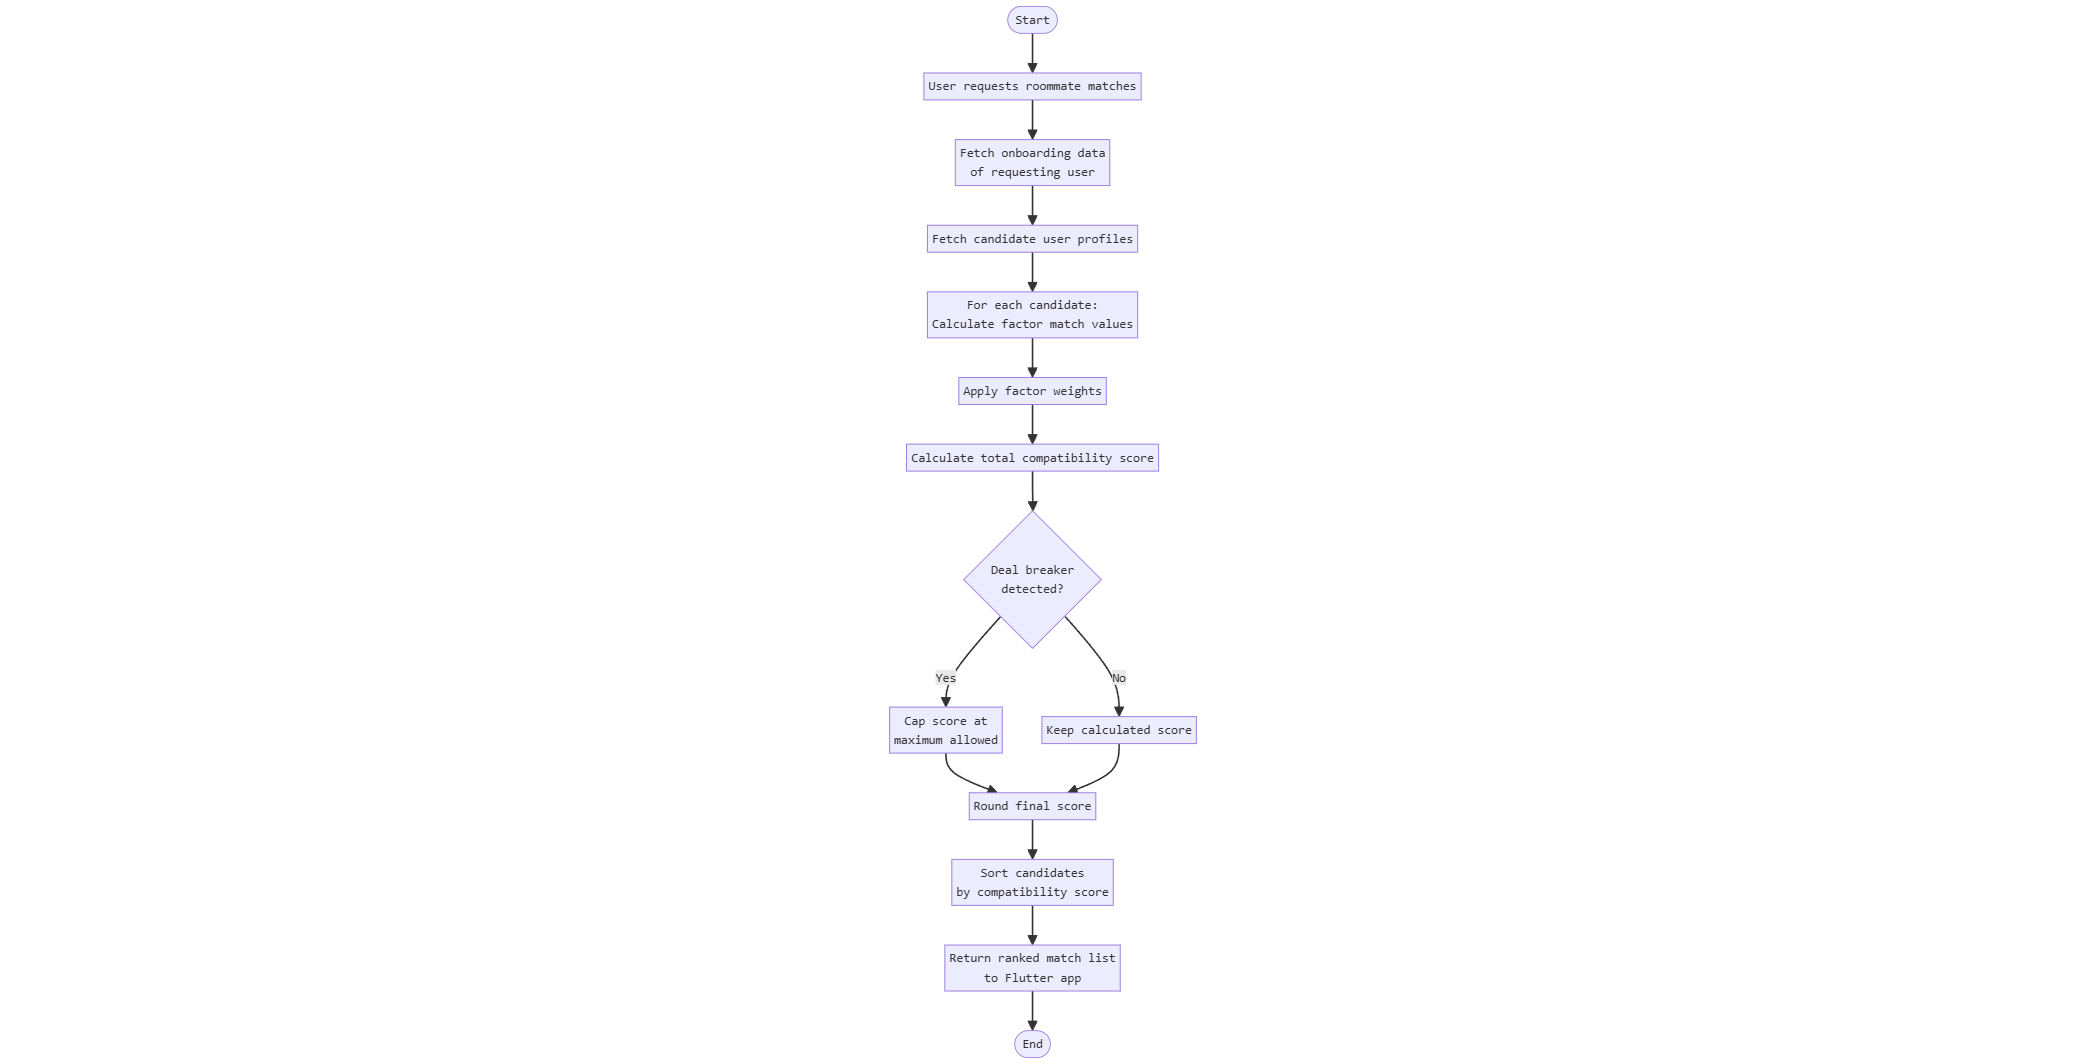
\includegraphics[width=1.0\textwidth, keepaspectratio]{images/flowchart.png}
    \caption{System Flowchart}
    \label{fig:flowchart}
\end{figure}
The flowchart illustrates the step-by-step operational flow of the TRIBAL system.


\section{UML Diagrams}
\begin{figure}[H]
    \centering
    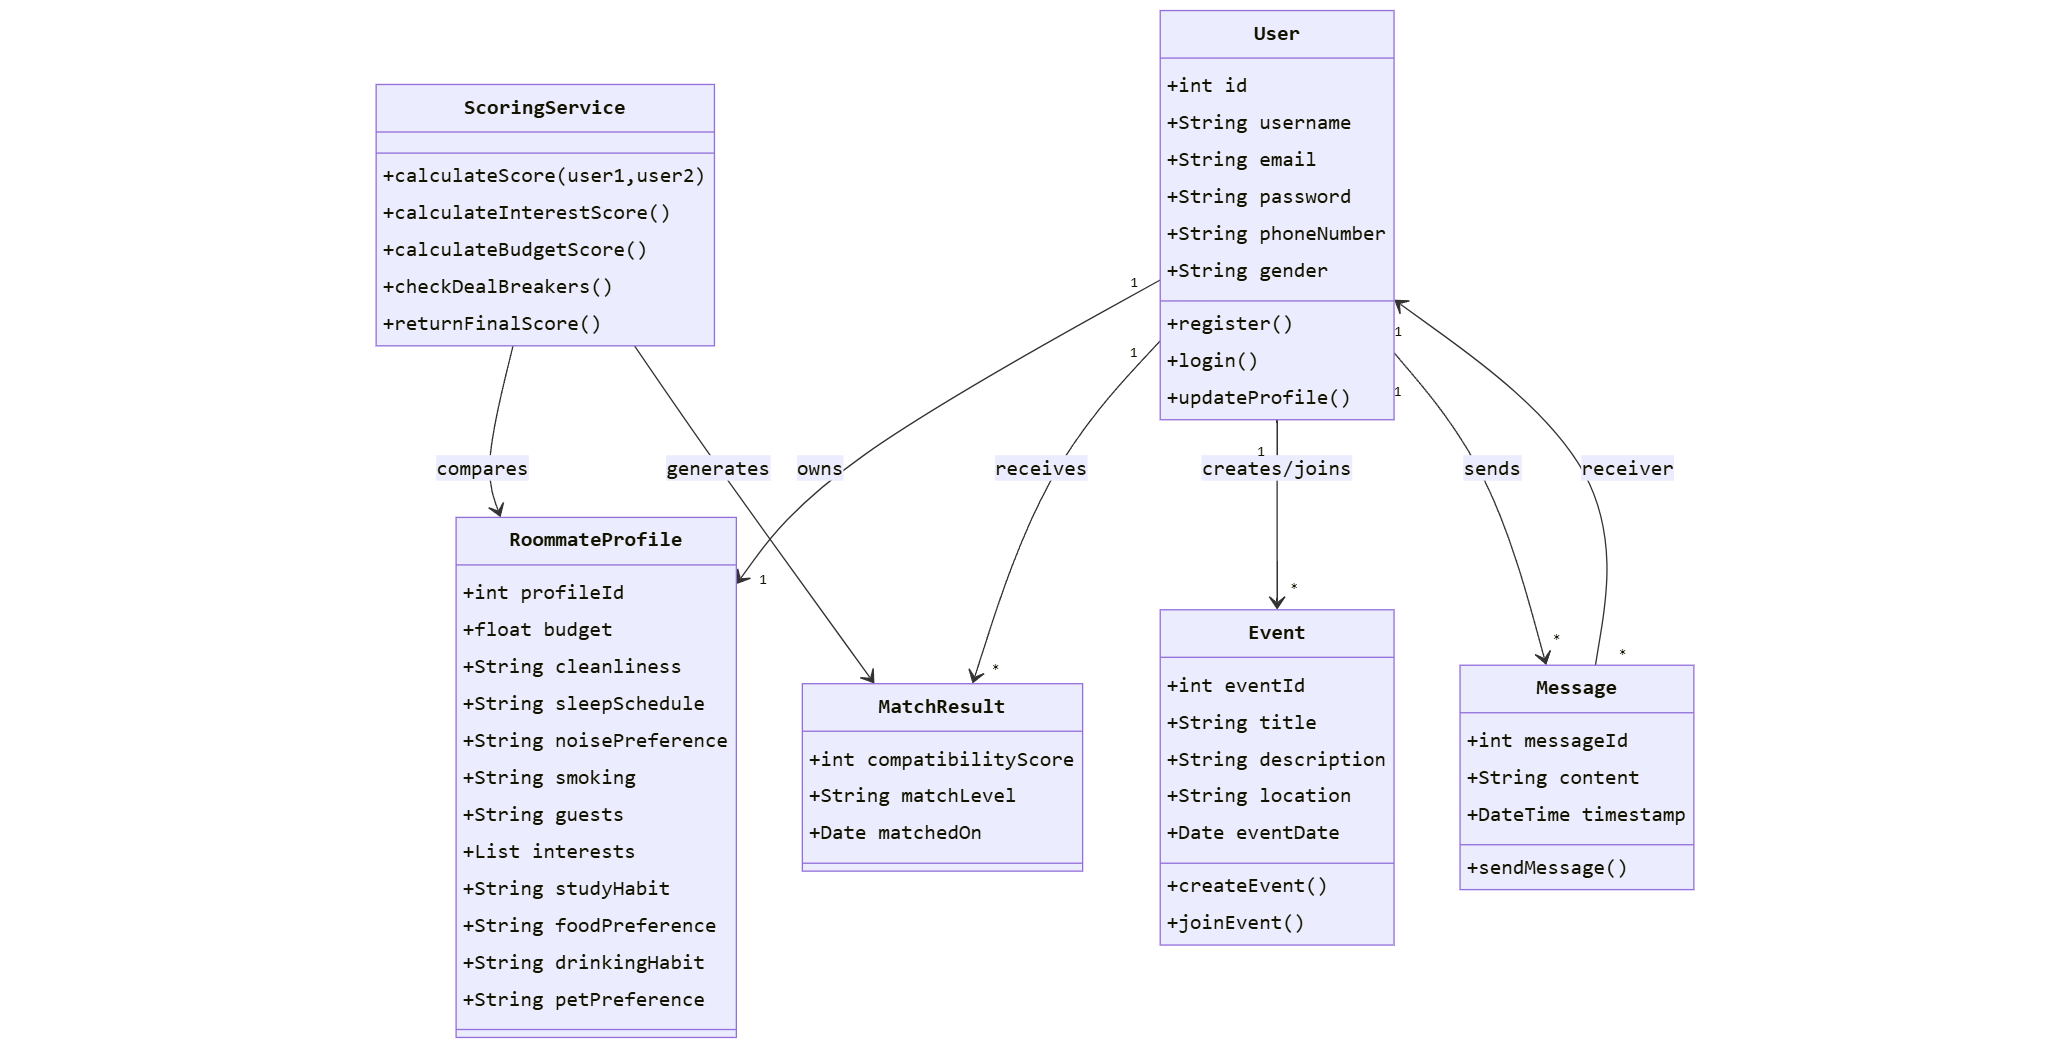
\includegraphics[width=0.95\textwidth]{images/uml.png}
    \caption{UML Diagram}
    \label{fig:uml_diagram}
\end{figure}
The UML diagram provides an object-oriented view of the system's architecture, showing key classes and their relationships.


\section{Tools Used}
The following tools and technologies are being used in the development of TRIBAL:
\begin{table}[H]
\centering
\begin{tabular}{|l|l|}
\hline
\textbf{Category} & \textbf{Tool / Technology} \\
\hline
Frontend Framework &  Flutter \\
Frontend Language &  Dart \\
State Management &  Provider \\
Navigation &  GoRouter \\
Backend Framework &  Django \\
Backend Language &  Python \\
Database &  PostgreSQL \\
Authentication &  JWT \\
Real-Time Communication &  Django Channels, WebSockets \\
Version Control &  Git, GitHub \\
Code Editor &  Visual Studio Code \\
Mobile Testing &  Android Studio \\
API Testing &  Postman \\
UI/UX Design &   Figma \\
\hline
\end{tabular}
\caption{Tools and Technologies Used}
\label{table:tools_used}
\end{table}
Flutter was chosen for the frontend because it allows the team to write one codebase that works on both Android and iOS. Django was chosen for the backend because it comes with many built-in features like an ORM and an admin panel, which makes development faster for a project with this scope. PostgreSQL was chosen as the database because it works well with Django and can reliably handle relational data like user profiles and onboarding responses.
